\chapter{Development}
This chapter describes in detail the main components of the simulation and how
they where implemented. How and why certain decision have been taken and alternative
solutions.

The project was developed in an iterative fashion, starting out with a
prototype and a reduced model, that has been redesigned and improved in small steps.

Presented here is the final solution developed during the thesis.

\subsection{Unity3d}
As mentioned before, Unity3d\footnote{Developed by Unity Technologies and available from https://unity.com}
is the game engine that has been chosen to implement the simulation. Unity3d is one
of the most popular game engines, and has been used to develop not only triple A
computer games but as well is applied more and more to build simulations for commercial and academic purposes.
Unity3d is distributed under various licencees, including a free of costs license, which
enables its use for Indie Game Developers as well to be applied in Academia.

\bb

For our purposes Unity3d is a generic simulation framework that provides the tools
to create virtual 3d environments, a physics engine, a user interface and autonomous
agents. The simulation is implemented as a Unity3 application with a single scene
that is dynamically generated based on the simulation and classroom configuration.

All objects (Agents and Tables) in the classroom are Unity GameObjects that are
updated in defined sequence with a constant rate of 1 Hz. The agent logic is therefor
running in discrete steps, although the underlying Unity3d engine is executed
continuously (as much as this is possible on a discrete computer system).

During development it was taken care to as much as possible separated, simulation logic
from Unity specific elements like visualization, or digital content management,
in order to reduce dependence and reusability of the system. The simulation logic
is implemented as C\# scripts that interface the Unity3d Framework.

\section{Agent-based model}
As described briefly in the chapter on the State of the Art (\ref{StateOfTheArt})
a agent-based model is a multi agent simulation with a special focus on the interaction
of agents and resulting group dynamics. The main components of a Agent-based
model are the following:

\begin{itemize}
    \item \textbf{the environment:} The environment is a strictly
    defined space in which the agents can move and interact with each other as 
    well as with other objects that are part of the environment. 
    \item \textbf{the agents:} The agents are autonomous dynamic systems with certain
    properties, sensors and actors that interact with each other and with the environment.
    \item \textbf{the simulation mechanics and agent logic:}  The simulation mechanics
    controls how agents interact with each other, how the environment changes
    as of actions of the agent or external factors (e.g. a simulation protocol defining
    a change in the environment). The agent logic governs the dynamic interaction between
    the internal agent state, its behavior and its properties.
\end{itemize}

\subsection{The environment: a classroom}
In our case the environment is classroom that contains multiple tables for
students to study individually and in small groups. In addition the environment
is modeling the noise that is accumulating in the classroom resulting from the
different actions performed by the agents. The noise model implemented, is
accumulating the noise produced by the different actions
performed by all agents in the classroom, whereby different Actions produce different
amount of noise depending on the simulation configuration.

Agents are moving about in the classroom as part of the various actions they perform.
The Unity3d Navigation Agent Infrastructure is used to control the movement of agents,
including path finding and collision control.

\label{agent}
\subsection{The agents: school children}

\begin{figure}[]
    \centering
    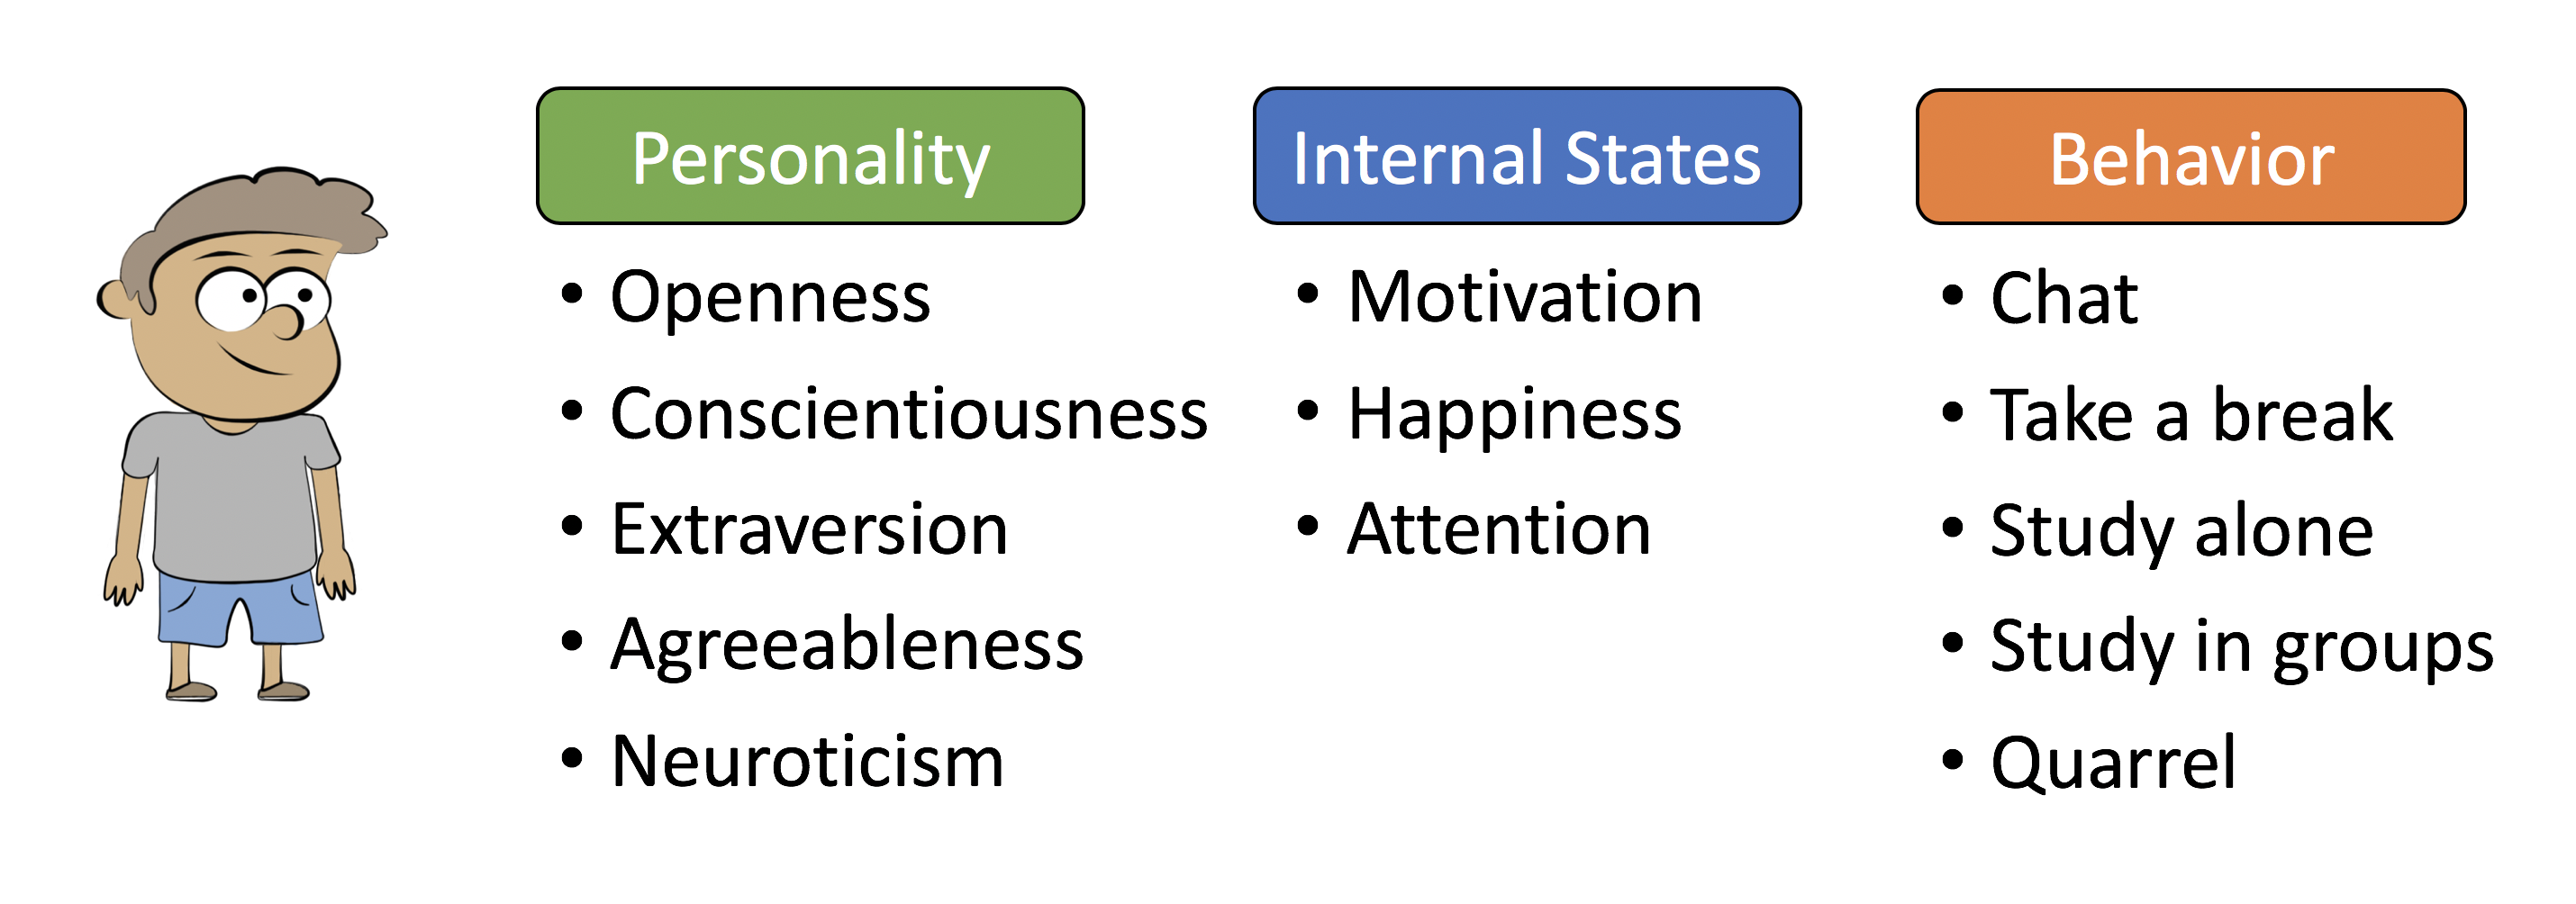
\includegraphics[width=400pt]{AgentOverview}
    \caption{Agent Overview}
    \label{AgentOverview}
\end{figure}

The agents are modeled to simulate school children of no specific age or physical
property. Instead agents are characterized completely by their personality traits
based on the Big Five Personality Traits model (see \ref{BigFive}). In addition
agents have several internal states and a set of possible behaviors they can perform (see \ref{AgentOverview}).

The internal states modeled by the agent are \textbf{motivation} to study, \textbf{happiness}
and \textbf{attention} during studies.

The behaviors available to the agents fall into one of three different types, being
either educational, recreational or aggressive.

\begin{itemize}
    \item \textbf{Chat:} Agents chat with another random selected agent in the classroom.
    \item \textbf{Take a break:} Agents take a break and start a random walk through the classroom.
    \item \textbf{Quarrel:} Agents start to quarrel with another random selected agent in the classroom.
    \item \textbf{Study alone:} Agents sit down on one of the individual tables and study by themselves.
    \item \textbf{Study in groups:} Agents take a spot on a group table and study with the other agents on the table.
\end{itemize}

Actions themselves have states, and an agent is always performing a single action
in a specific state

\begin{itemize}
    \item \textbf{Inactive:} The action is not active (This is needed because of implementation details). 
    \item \textbf{Transition:} The agent is walking towards its goal to in order to perform the action.
    \item \textbf{Waiting:} The agents is waiting for either some response of another agent or the environment in order to perform the action.
    \item \textbf{Executing:} The agent is executing the action.
\end{itemize}

As the agents behavior depends on the internal states but as well is effecting them,
each agent itself is a \textbf{dynamics systems} that is governed by the agent logic, based
on the personality profile of the agent (see a visualization of this cycle in figure \ref{AgentDynamics}).

\begin{figure}[]
    \centering
    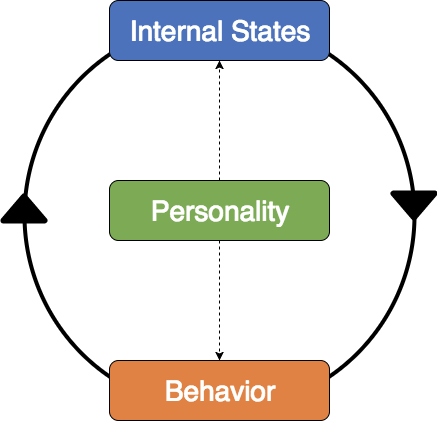
\includegraphics[width=200pt]{AgentDynamics} 
    \caption{Agent Dynamics}
    \label{AgentDynamics}
\end{figure}

\subsubsection{Dynamic Systems}
As mentioned in the introduction, agent-based models are focus on the interaction
\textit{between} components of the simulation. As we have shown that the agents
are themselves dynamics systems, complete system is therefore the result of the
interaction of multiple dynamic systems (i.e. agents and environment)
(see figure \ref{GroupDynamics}). 

\bb

This \textbf{multi level dynamic system} can express very sophisticated behavior and dynamics,\
making it one of the main reasons agent-based models are such a powerfully tool to study
real world social phenomena. One of the most curious aspects of complex dynamic systems
are \textbf{emergent phenomena}\cite{Corning2002} which describe aspects of the
complete system (i.e. classroom), absent in the individual (i.e. children) components.

\bb

One examples of emerging properties is the \textit{wetness} of Water that only appears in a
ensemble of many water molecules, and not present in a single individual molecule. 
Another famous example is \textbf{Cowans Game of Life}\cite{Adamatzky2010}
that shows the almost infinite complexity generated by a cellular automata simulating
black or white cells on a infinite grid. Constructs generated by the simulation
have emerging properties like \textit{self replication}, \textit{finite} and
\textit{infinite life cycles} and many more. None of those behaviors are obviously deducible
from the initial basic interaction rules. Instead those properties emerge in the
interaction between the components or agents following basic rules.

\begin{figure}[]
    \centering
    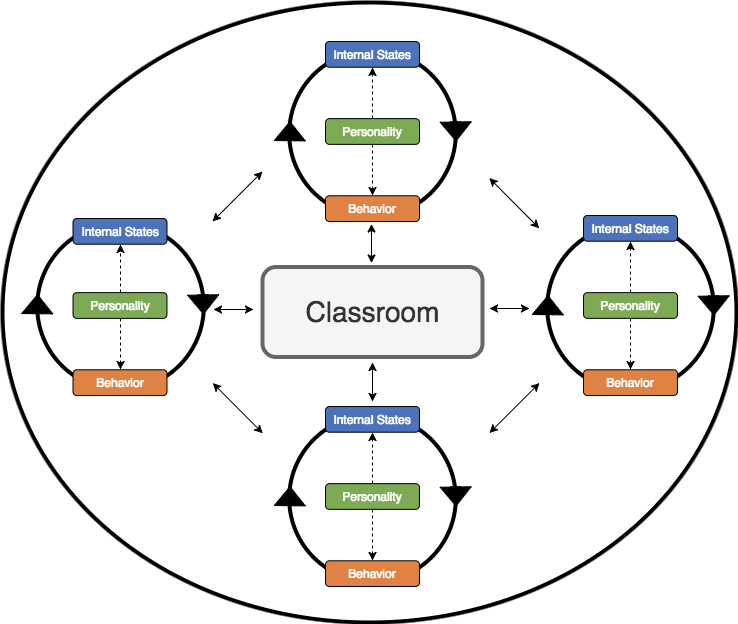
\includegraphics[width=400pt]{GroupDynamics} 
    \caption{Group Dynamics}
    \label{GroupDynamics}
\end{figure}

\subsubsection{Agent homogeneity}
One important axis along which to classify agent-based models is agent homogeneity\cite{Pudane2017}.
In homogeneous agent models all agents share the same characteristic's and agent logic.
Heterogeneous agent models on the other side can differ in the agents logic, its behavior
or based on some parameters in its configuration.

In our case the simulation contains heterogeneous agents that differ, based on parameters
in their Personality Traits. All agents follow the same logic and have teh same
capabilities.

\subsection{Agent Behavior Selection}
The following are the different factors that influence agent behavior:

\begin{itemize}
    \item \textbf{Environment:} The availability of tables, and the accumulated noise in the classroom. 
    \item \textbf{Direct agent interaction:} Another agent that accepts ot rejects to chat or quarrel with he agent.
    \item \textbf{Internal states:} Based on internal states agent logic governs which action is more or less desired by the agent.
    \item \textbf{Peer Pressure:} The action an agent selects to perform is influenced on the average action preference of the group.
\end{itemize}

How peer pressure is modeled is discussed in more detail in \ref{action-scores}.


%%%%%%%%%%%%%%%%%%%%%%%%%%%%%%%%%%%%%%%%%%%%%%%%%%%%%%%%%%%%%%%%%%%%%%%%%%%%%%%%
\pagebreak

\label{BigFive}
\section{Agent Personality Model}
As described earlier agents differ between each other only in their Personality, 
witch is modeled on a set of \textbf{Personality Traits}.

It is not novel to use personality traits in ABM, but previous works\cite{Gautam2009}
modeled very abstract personality traits that have no psychological bases.

We therefore where careful, to chose an established and widely used personality traits model.
The \textbf{OCEAN} personality trait model(\cite{Tupes1961}, \cite{John1999}), common known as the \textbf{Big-Five}, has been developed
in the 1960s and has since been used in applied and theoretical psychology.
It is based on factor analysis of empirical studies (mostly self description of patients about their
behavior and self image).

\section{The Big-Five}
Its name is derived from the five orthogonal dimensions which are used to describe
the personality of an individual, whereby the extremes of each dimension are associated
with typical behaviors or thought patterns (see figure \ref{OCEAN-Model} for a graphical
summary).

A short description of the different dimension been taken from\cite{Ehrler1999}
can be found in the table \ref{OCEAN-Model-table}.

\subsection{Stability of Personality Traits}
From the literature it is not clear how stable the personality traits described
by the OCEAN model really are. Some studies (\cite{Srivastava2003} \cite{Soto2011}) 
show gender differences and systematic changes of traits during the lifetime of 
a person, and specially during adolescence. Other studies on the other side, found
results(\cite{Soldz1999}, \cite{Cobb-Clark2012}) on the stability of personality traits for a very long time or even the
complete life or an individual.

\bb

Independent of their stability over time, personality traits seem not to depend on
hereditary factors alone, as studies\cite{Deckers2015} show different life factors like socio-economic status
to be a powerful predictor of personality traits.

\bb

The concrete origins and dynamics of personality traits go beyond this work, and
we decided there is enough evidence in the literature to justify the OCEAN
model as a useful personality model and the personality traits are stable enough
to be taken as constant for your purposes.

\begin{figure}[h]
    \centering
    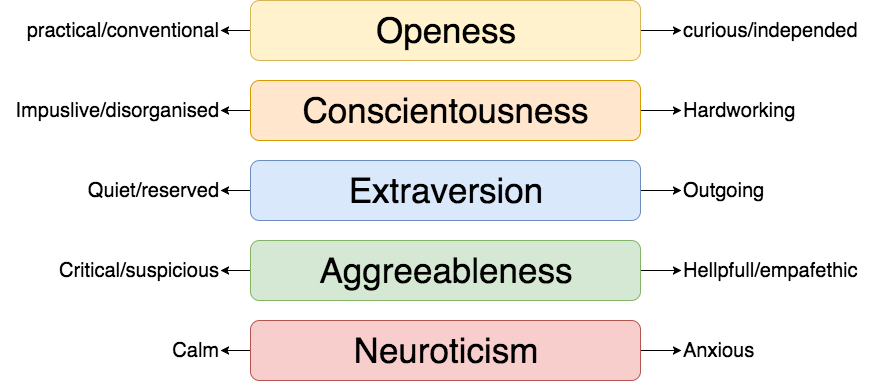
\includegraphics[width=400pt]{OCEAN-model} 
    \caption{OCEAN Model}
    \label{OCEAN-Model}
\end{figure}

\begin{table}[]
    \makebox[\textwidth][l]{%
    \begin{minipage}[t]{10cm}
\begin{tabularx}{1.6\textwidth}{|>{\hsize=.2\hsize}X|X|}
    \hline
    \multicolumn{1}{|c|}{\textbf{Personality Trait}} & \multicolumn{1}{c|}{\textbf{Description}} \\
    \hline
    
    Openess & The general tendency to be curious about both inner and outer worlds.
    O includes the elements of an active imagination, aesthetic sensitivity,
    attentiveness to inner feelings, preference for variety, intellectual
    curiosity, and independence of judgment. A high O also includes individuals
    who are unconventional, willing to question authority, and ready to entertain
    new ethical and social ideas. \\
    \hline
    
    Conscientiousness & The general tendency to be able to resist impulses and
    temptations. The conscientious individual is purposeful, strong-willed, and
    determined.
    On the positive side, high C is associated with academic and occupational
    achievement; on the negative side, it may lead to annoying
    fastidiousness, compulsive neatness, or workaholic behavior, Low C’s are not
    necessarily lacking in moral principles, but they are less exacting
    in applying them. \\
    \hline
    
    Extraversion & The general tendency to be outgoing. In addition, high E’s
    prefer large groups and gatherings and are assertive, active, and talkative.
    They like stimulation and tend to be cheerful in disposition. They are upbeat,
    energetic, and optimistic. \\ 
    \hline
    
    Agreeableness & The general tendency to be altruistic. The high A is
    sympathetic to others and eager to help them, and believes that others will
    be equally
    helpful in return. By contrast, the low A is antagonistic and egocentric,
    skeptical of others’ intentions, and competitive rather than cooperative. \\
    \hline
    
    Neuroticism & The general tendency to experience negative affects such as fear,
    sadness, embarrassment, anger, guilt, and disgust is the core of the N domain. 
    However, N includes more than susceptibility to psychological distress. Perhaps
    because disruptive emotions interfere with adaptation, those
    who score high in N are also prone to have irrational ideas, to be less able
    to control their impulses, and to cope more poorly then others with stress. \\
    \hline
  \end{tabularx}
  \label{OCEAN-Model-table}
  \caption{Ocean model factors taken from \cite{Ehrler1999}}

\end{minipage}    
}%
\end{table}

\subsection{Big-five in the classroom}
Various empirical studies have been performed in the past in order to investigate
the association between Personality Traits, behavior and academic outcome in schools
(\cite{Ehrler1999}, \cite{Nigg2002}, \cite{Asendorpf2003}).
We used those empirical found associations to define and tune agent logic as well
as simulation parameters in order to reproduce agent behavior that is in agreement
with those results.

As a summary of those findings we cite from \cite{Asendorpf2003} where the authors
write.

\bb

\textit{Together, this literature review suggested the following hypothesis:
neuroticism and low extraversion correlate with social inhibition, low agreeableness
and low conscientiousness with aggressiveness, and conscientiousness and
culture/intellect/openness with antecedents and outcomes of school achievement.
These correlations are consistently found all throughout childhood.}

\bb

Although it is well studies how the Big-Five behave on an individual level, we
found very few studies that focused on group dynamics influenced by the
Big-Five. One work that we did find\cite{Selfhout2010} studied how the Big-Five
influence the forming of new friendships in adolescence, but limited the study
to pair wise interactions.

Another study \cite{Golsteyn2017} showed the effect of personality traits of members
in a peer group on the academic achievement of the individuals. The investigators
defined their own academic relevant personality traits and showed how more persistent
peers elevate the academic performance of less persistent peers without costs to
those peers or themselves.

To the best of your knowledge there is no previous work that uses the Big-Five
personality trait model to studies how group dynamics in a classroom are affected
by different personality profiles.

\subsection{Alternatives to the Big-Five}
The Big-Five model is not the only popular personality trait model commonly used.
Another model, specially popular in the area of management and labour market, is the
Myers Briggs Type Indicator \textbf{MBTI}, which assigns each individual to one
of 16 possible personality types. Although popular, there seems to be no scientific
basis for the model and scientific investigation into it\cite{Pittenger1993}
revealed low predictive power and accuracy of the model.

\bb

The OCEAN model has therefore been preferred over any alternative.

%%%%%%%%%%%%%%%%%%%%%%%%%%%%%%%%%%%%%%%%%%%%%%%%%%%%%%%%%%%%%%%%%%%%%%%%%%%%%%%%
\pagebreak

\section{Agent Logic}
As mentioned before the simulation is using a heterogeneous agent model with agents
differ in their personality traits, but share the same logic and capabilities.

The logic is executed independently on each agent, and is implemented as a infinite
loop, repeating the following steps

\begin{enumerate}
    \item \textbf{Calculating action scores}
    \item \textbf{Action selection}
    \item \textbf{Action execution}
    \item \textbf{Handling interactions}
    \item \textbf{Updating internal states}
\end{enumerate}

\subsection{Calculating action scores}
The agent can execute one of five actions (see the section \ref{agent} about available actions).
In order to decide witch action to execute, a score is calculated for each action independently.
Section \ref{action-scores} covers the action score calculation in detail. 
The score of an action depends on the the internal states of the agent and its
psychological profile.

\subsubsection{Action Score Bias}
Besides the action score, the agent is calculating an \textbf{action score bias}
that is added to the score of the current action and subtracted from the score
of the previous action. This mechanism is used to keep the agent from switching
between actions too quickly. In addition, the added bias models the tendency to
continue with an ongoing task and switching costs between tasks (similar to sustaining attention).
Reducing the score of the previous action keeps the agent from looping between two
of the possible actions, and cause a more diverse action selection.

\bb

The action score bias depends on the conscientiousness of the agent and is following an
exponential decay curve, where time is the number of ticks the agent is performing
the current action. The number of ticks is only taken into account while the action is executed,
not in its other states, making sure that \textit{Transitions} or \textit{Waiting}
do not effect the action score bias.

\begin{equation}
    \label{eq1}
    action-score-bias(a_i) = \alpha * e^{-(1.0 - C) \beta * t}
\end{equation}
with
\begin{itemize}
    \item $a_i$ is the action i
    \item where $\alpha$ is a simulation parameter defining the maximum bias
    \item where $\beta$ is a simulation parameter defining a dampening factor scaling exponential decline
    \item where C is the agents conscientiousness
    \item where t is the number of ticks the current task is executed
\end{itemize}

\subsection{Action selection}
Based on the scores a single action is selected probabilistically, giving preference
to the action with the highest score.
The probability for a action to be selected is defined by the square of the normalized
action scores (see equation \ref{eq2}). Taking the squared action score makes sure
that the highest rated score has a clear advantage over the other actions, but still
gives other actions a chance to be selected.

\begin{equation}
    \label{eq2}
    p(a_i) = \frac{s_i^3}{\sum s_i^3} \\
\end{equation}

with
\begin{itemize}
    \item $p(a_i)$ is the probability of action i to be selected
    \item where $s_i$ is the score for action i
\end{itemize}


\subsection{Action execution}
The selected action it is evaluated if it can be performed, and if this is possible
than the action is executed. If the action cannot be performed, the agent is forced
to take a break, which works as the default action. In addition if it is not possible
to perform an action, the agent keeps track of what its desired action is, and what
the action that it is executing instead. 

\subsection{Handling Interaction}
Some of the agent behaviors like \textit{Chat} and \textit{Quarrel} depend on direct
interactions between agents. Meaning that if agent A want to chat with agent B (who is
randomly selected from the available agents), than Agent A depends on B
\textit{accepting} its invitation to chat. This mechanism is implemented
by agent A is sending a request for chatting to agent B, and agent B in return
decides to either accept or reject the invitation. 

In case the request is accepted both agents perform the action (i.e. Agent B will
interrupt its current action), and if rejected, the sending agent A will retry either
sending another request to the same agent B, or start over with another agent.

\bb

Agent B decides its response depending on a random factor and its personality traits.
In case of chat the relevant personality trait is \textit{conscientiousness} and
in case of quarrel \textit{agreeableness}. The random factors is a number between 0.0
and 1.0 that is randomly generated and compared to the personality trait.
Is that number equal or bigger than the corresponding personality trait, the agent
will accept the interaction.

\bb

This mechanism reflect the empirical findings that agents with a high level of
conscientiousness are less likely to be distracted from the their current task,
and high level of agreeableness, reducing the chance to quarrel, as it is associated
with less involvement in conflicts.

\subsection{Updating internal states}
At the end of each cycle, the agent is updating its internal states, whereby
from the three internal states (i.e. motivation, attention and happiness), only attention
and happiness are updated at this point.

\begin{itemize}
    \item \textbf{Happiness:} is increased if the current action is not quarrel,
    and the executed action is the desired action. In case the agent
    is executing a not desired action happiness is decreased by a factor (a
    simulation parameter) that is scaled by the agents neuroticism. In addition
    happiness is effected by the different actions (discussed later).
    \item \textbf{Attention:} is calculated in case the agent is studying (either
    alone or in a group). It is calculated by taking the sum of its motivation
    adding conscientiousness and subtracting the noise in the classroom.
\end{itemize}

As \textit{motivation} is concerned, this internal state is altered by the current action performed.

\section{Actions}
As mentioned before, agents have the capability to perform one of five actions (i.e.
Chat, Quarrel, Break, Study alone and Study in groups),
with each action being in one four states (Inactive, Transition, Waiting and Execution)
at each moment in time.

All actions follow a similar structure, and have three main functions:

\begin{itemize}
    \item \textbf{Test Feasibility:} Test if it is possible to execute and action. This
    includes to test for the availability for resources in the environment
    (e.g. for example if there is a free individual table for a agent to study alone)
    or the availability of other agents (e.g. in case of a group study if there are
    other agents at the table willing to study).
    \item \textbf{Action scoring:} Calculates a score for the action based on the
    internal states and the personality of the agent.
    \item \textbf{Action execution:} Makes the agent perform different behaviors
    based on the state of the action (e.g. in Transition it makes the agent walk toward its goal).
    This is the point in which the internal state motivation is altered according
    to the simulation mechanics.
\end{itemize}

Before describing the exact mechanics for the different action we have a look at
how to calculate the action scores.

%%%%%%%%%%%%%%%%%%%%%%%%%%%%%%%%%%%%%%%%%%%%%%%%%%%%%%%%%%%%%%%%%%%%%%%%%%%%%%%%

\pagebreak
\label{action-scores}
\section{Actions Scores}
As mentioned before each action is scored independently, taking into account the
internal states and the personality traits of the agent. The score calculate reflects
how appropriate the specific action is for the personality and the internal state
of the agent.

The generated score is a continuos value between 0 and 1.0, where high values
are given if the actions is in correspondence with the simulation mechanics, and
low values otherwise.

Although the scoring differs between the specific actions, all of them make use
of the same basic building blocks.

\bb

Those blocks are an exponential growing, an exponential decaying function and a
function calculating the weighted sum of three components (see equation \ref{eq3}
and a visualization in figure \ref{Equatin_figures}). The weights for the sum correspond
to the importance given to personality, motivation and happiness in calculating the score.
The weights are simulation parameters and stay constant for the simulation. The components summed
are the exponential growing or decaying function, depending on the internal state
and the personality of the agent.

The exponential functions have been defined to stay within a range of 0.0 to 1.0
for values of x between 0.0 and 1.0. In addition, the result of the scoring function
is cutoff to stay within 0.0 and 1.0.

\bb

As mentioned before, the internal states happiness and motivation are effected by
the action the agent is performing. How the internal states are effected, depends
on the state of the action, and differs between \textit{Waiting, Transition} and \textit{Execution}.
Where for \textit{Waiting} and \textit{Transition} the effect strength on happiness is modulated
by the agents neuroticism and agreeableness, and during \textit{Executing}
motivation and happiness are changed by a constant factor that is defined as a
simulation parameter.

\begin{subequations} 
\label{eq3}
\begin{equation}
    E_{grw}(x) =  \frac{e^{x^2}-1}{e - 1}
\end{equation}
\begin{equation}
    E_{dec}(x) =  \frac{e^{(1 - x)^2}-1}{e - 1}
\end{equation}
\begin{equation}
    weighted_sum(\alpha,x,\beta,y,\gamma,z) = (\alpha * x) + (\beta * y) + (\gamma * z)
\end{equation}
\end{subequations}
with
\begin{itemize}
    \item $\alpha$ the weight of personality
    \item $\beta$ the weight of motivation
    \item $\gamma$ the weight of happiness
\end{itemize}

\begin{figure}[!h]
    \label{Equatin_figures}
    \makebox[\textwidth][l]{%
        \begin{minipage}[t]{4cm}
            \centering
            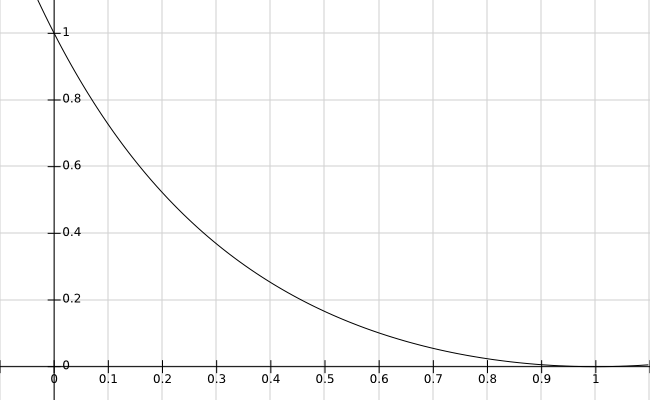
\includegraphics[width=200pt]{ExpDecay}
            \caption{Exponential Decay}
        \end{minipage}
        \hspace{3cm}
        \begin{minipage}[t]{4cm}
            \centering
            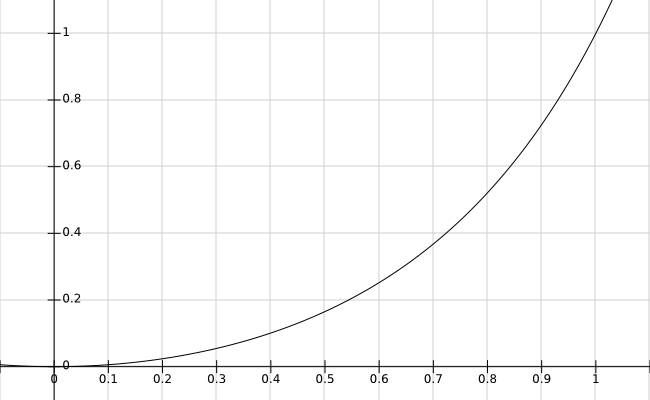
\includegraphics[width=200pt]{ExpGrowth}
            \caption{Exp Growth}
        \end{minipage}
    }%
\end{figure}

\subsubsection{Chat}
The intention of \textit{Chat} is to recover the motivation of the agent, preferred
by agents with high rates on extroversion. In order to chat, the agent will
randomly select another agent in the classroom to chat with, and approach that agent.
If the other agent accepts the invitation, and both agents are next to each other,
the agents will start chatting. If the request was rejected, the agent will repeat
to send requests for a specific number of times to, before giving up and choosing
another agent to start over.

The action scored is calculated using the following scoring function

\begin{equation}
    weighted_sum(extroversion, w_{per}, E_{dec}(motivation), w_{mot}, E_{grw}(happiness), w_{hap})
\end{equation}

While the agents are chatting, they will produce a bit of noise adding the
accumulated noise the classroom.

\subsubsection{Takeing a break}
The intention of this action is to recover motivation of the agent, for individuals
with low rates on extroversion, working as an alternative to chatting.
When taking a break, agents don't depend on any other agent, and will start to
wander around in the classroom randomly, performing a random walk, causing no noise
while doing so.

The action scored is calculated using the following scoring function

\begin{equation}
    weighted_sum(1.0 - extroversion, w_{per}, E_{dec}(motivation), w_{mot}, E_{grw}(happiness), w_{hap})
\end{equation}

\subsubsection{Quarrel}
Quarreling is the result of an agents happiness being very low and being at least
medium to highly motivated. In order to quarrel the agent has to find another agent
to do so. Similar to Chat the agent will select another agent randomly and starts
to quarrel with that agent if accepted. If the other agent refuses, the unhappy
agent will repeat its request a fixed number of times before searching for another agent.

Once the agents start quarreling, their motivation and happiness will fall drastically.
In addition quarreling produces a lot of noise that is added to the accumulated
noise in the classroom.
When the agents stop to quarrel as special mechanism is invoked, immediately
increasing the happiness of the agents by a fixed value (simulation parameters).

The action scored is calculated using the following scoring function

\begin{equation}
    weighted_sum(agreeableness, w_{per}, E_{grw}(motivation), w_{mot}, E_{dec}(happiness), w_{hap})
\end{equation}


\subsubsection{Studying alone}
If the agent is motivated and happy, it will start to study, preferring
to study alone in case of low levels of extroversion. In order to study alone the
agent needs access to a free individual table, and that the noise in the classroom
is not too high. The acceptable noise level for an agent is depending on its
conscientious, sustaining higher noise levels with higher rates of conscientious.
Studying alone increases noise levels slightly.

The action scored is calculated using the following scoring function

\begin{equation}
    weighted_sum(1.0 - extroversion, w_{per}, E_{grw}(motivation), w_{mot}, E_{grw}(happiness), w_{hap})
\end{equation}

\subsubsection{Studying in groups}
Agents with high extraversion rates, motivation and happiness, will start to study
in groups. What agents need to do so, is a seat on a group table and other agents
at the table that are willing to study. Groups studying increase the noise level
in the class by a medium amount.

The action scored is calculated using the following scoring function

\begin{equation}
    weighted_sum(extroversion, w_{per}, E_{grw}(motivation), w_{mot}, E_{grw}(happiness), w_{hap})
\end{equation}
